\section{Windows Logs}
\subsection{TLP (Traffic Light Protocol)}
\paragraph{TLP:RED}
Infos sind auf den Kreis der Anwesenden beschränkt. Eine Weitergabe ist untersagt.

\paragraph{TLP:AMBER}
Info darf der Empfänger innerhalb seiner Organisation auf Basis ``Kenntnis nur wenn nötig'' weitergeben.

\paragraph{TLP:GREEN}
Infos dürfen innerhalb der Organisationen und an deren Partner weitergegeben werden. Die Informationen dürfen jedoch nicht veröffentlicht werden.

\paragraph{TLP:WHITE}
(default) Abgesehen von urheberrechtlichen Aspekten dürfen Informationen ohne Einschränkungen frei weitergegeben werden.

\subsection{LSASS Process}
Local Security Authority Subsystem Service (LSASS) is a process in Microsoft Windows operating systems that is responsible for enforcing the security policy on the system. It verifies users logging on to a Windows computer or server, handles password changes, and creates access token. \\

lsass.exe is a Windows process that takes care of security policy for the OS. For example, when you logon to a Windows user account or server lsass.exe verifies the logon name and password. If you terminate lsass.exe you will probably find yourself logged out of Windows. lsass.exe also writes to the Windows Security Log so you can search there for failed authentication attempts along with other security policy issues.

\subsection{Event Log Format}
Event Logs are in the Binary Format and only written by the LSASS Process.
You have to open the Logs with the Event Viewer. If you open them with VS Code, the file is unreadable.\\

\subsubsection{Size and saveplace}
Every Log has a maximum size. The default is \textbf{20Mb}.
The default Log directory is: 
\begin{lstlisting}
  %windir%\System32\winevt\Logs\*.evtx
\end{lstlisting}
but it can be changed with the following registry key:
\begin{lstlisting}
  Computer\HKEY_LOCAL_MACHINE\SYSTEM\CurrentControlSet\Services\EventLog
\end{lstlisting}

\subsubsection{Categories}

\paragraph{Security.evtx}
\begin{itemize}
  \item Access control and security information
  \item Only Written by LSASS Process (based on GPO Settings)
  \item Security Event Log is most important for cyber defense
\end{itemize}

\paragraph{System.evtx}
Windows system events (such as driver, service and resource events).

\paragraph{Application.evtx}
Non-System related software events

\paragraph{Custom.evtx}
\begin{itemize}
  \item Around 150 different custom application logs (RDP, Powershell, Firewall)
  \item Big chances of retaining logs much longer than say Security
\end{itemize}

\subsubsection{Obtaining Security Logs}
Event Log files are usually locked when the system is in running!\\

\paragraph{Running System}
\begin{enumerate}
  \item Exporting Logs from Event Viewer
  \item PsLogList tool
  \item PowerShell (Get-WinEvent)
  \item Evtx Explorer / EvtxECmd by Eric Zimmermann
\end{enumerate}
\paragraph{Dead / Stopped System}
Copy the directory \%windir\/System32/winevt/Logs

\paragraph{Useful Commands}
\begin{lstlisting}
  Get-WinEvent -ListLog *powershell*
  Get-WinEvent -ListLog *security*
  Get-WinEvent -ListLog *firewall*
  Get-WinEvent -LogName 'Security' | Out-Host -Paging
  Get-WinEvent -FilterHashTable @{LogName='Security';ID='4625'} | Format-List
\end{lstlisting}

\subsection{Security Events}
\begin{itemize}
  \item System Events $\rightarrow$ System start / shutdown / \dots
  \item Logon Events $\rightarrow$ User logging on or off (stored on authorized system)
  \item Account Logon $\rightarrow$ Recorded on the authorizing system (Domain Controller usually)
  \item Privilege Use $\rightarrow$ User Account exercising a privilege
  \item Account Management $\rightarrow$ Modifications of accounts
  \item Object Access $\rightarrow$ System Access Control List (SACL) based objects (files / folders / registry)
  \item Directory Service $\rightarrow$ AD Object with SACL accessed
  \item Process Tracking $\rightarrow$ Process start, exit, \dots
\end{itemize}

\subsubsection{Event IDs}
\begin{itemize}
  \item 4720: Account Creation
  \item 4624: Successful Logon
  \item 4625: Failed Logon
  \item 4624 / 4647 / 4634: Successful Logoff
  \item 4738: A user account was changed (permissions granted or similar)
  \item 4648: Logon with explicit credentials
  \item 4776: Local account authentication (NTLM authentication)
  \item 4672: Special privileges assigned to new logon
  \item 4779: A user disconnected a terminal server session without logging off.
\end{itemize}

\paragraph{Logon Type}
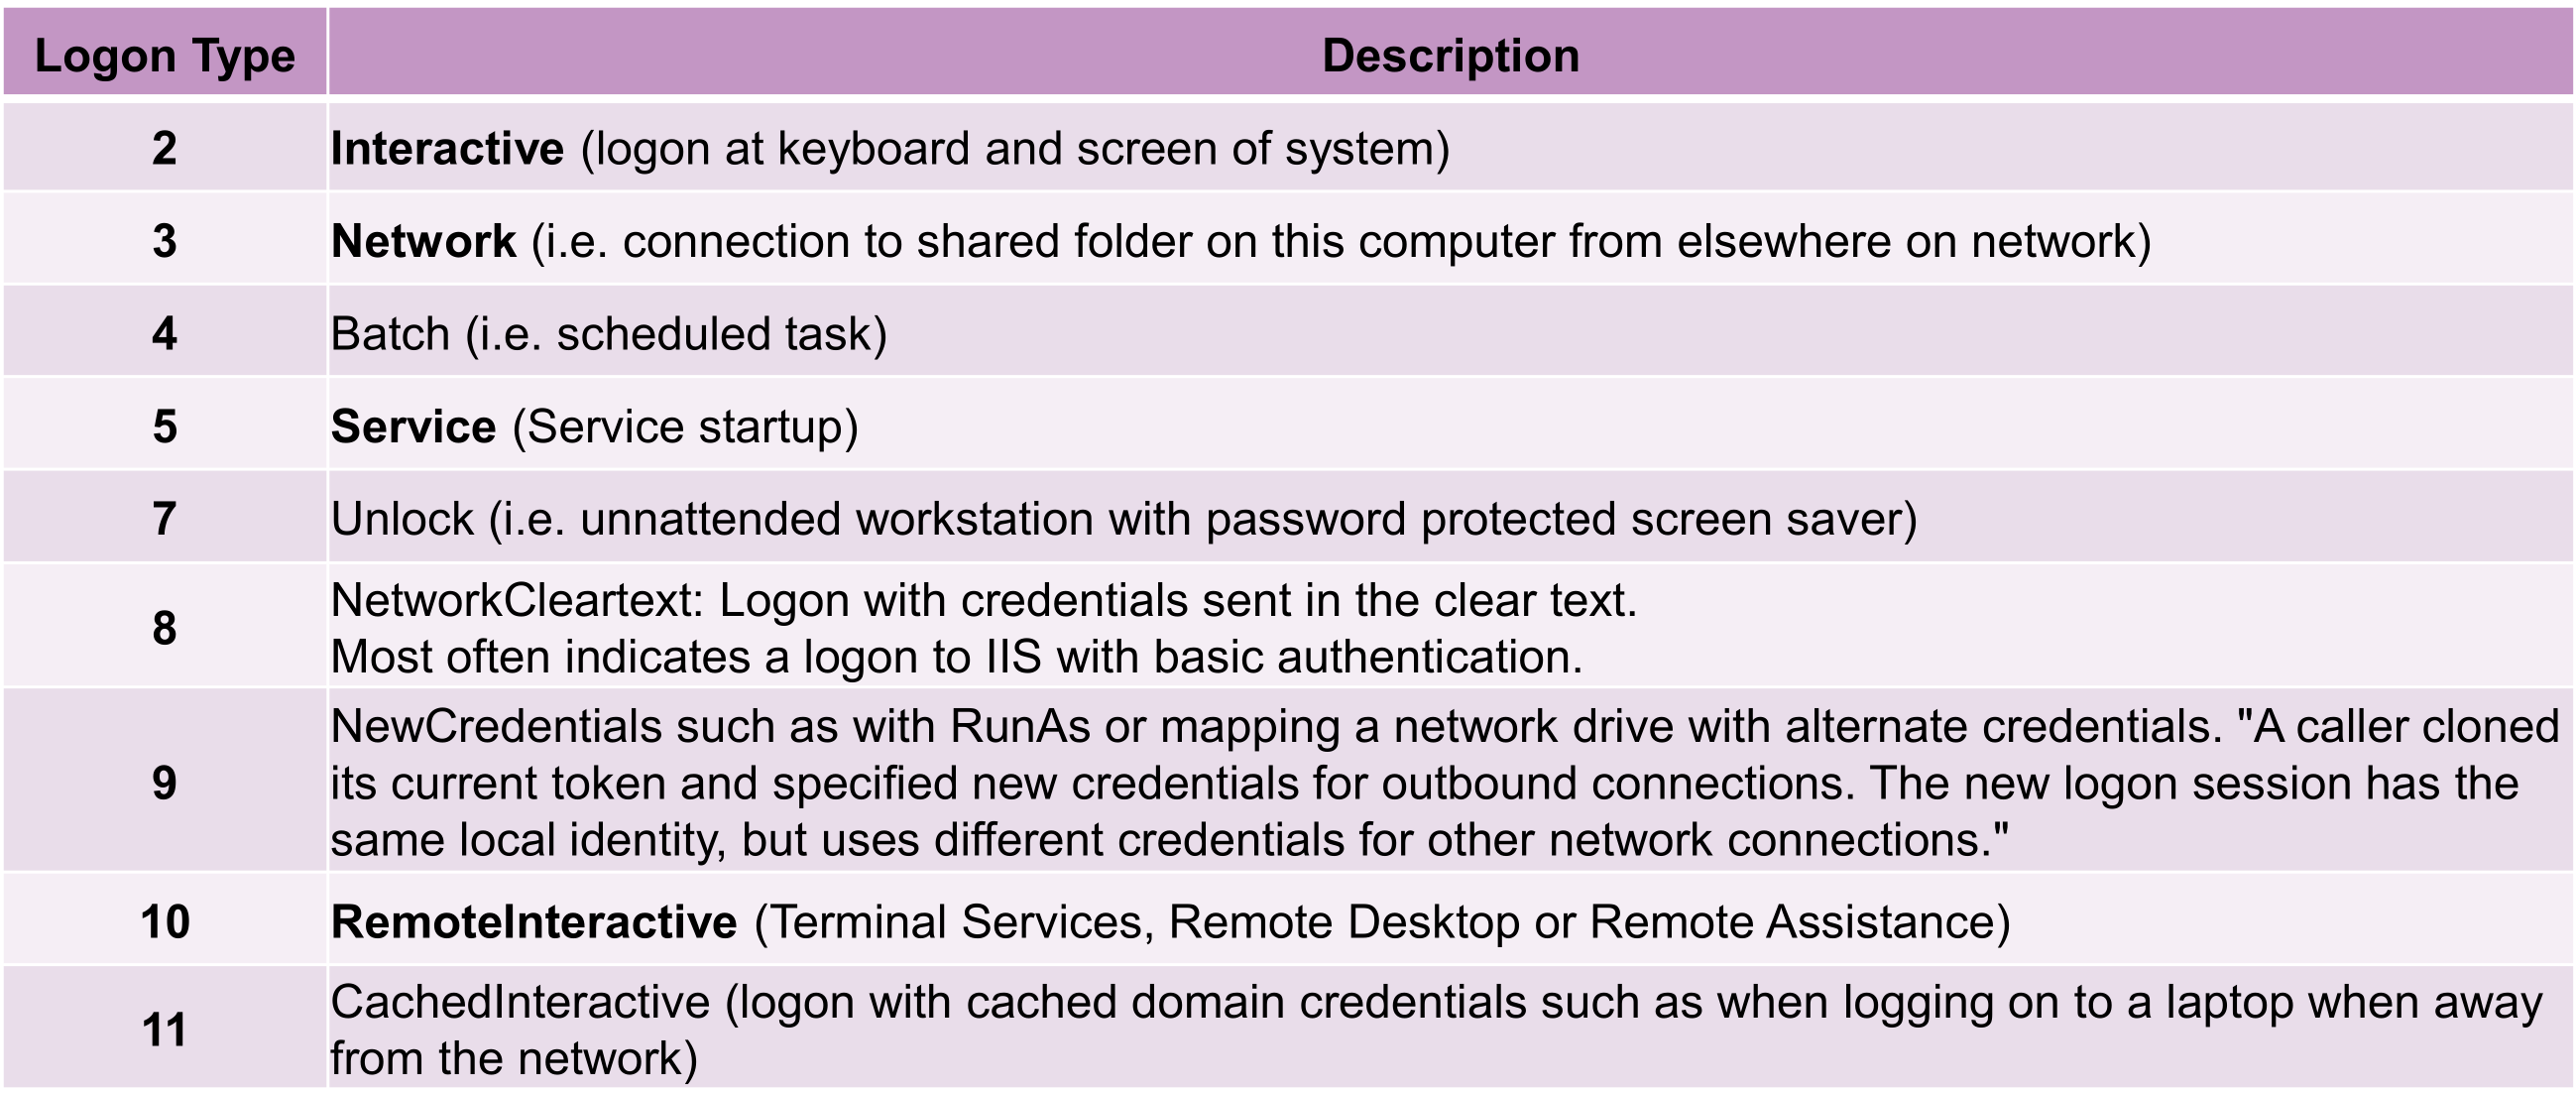
\includegraphics[width=\linewidth]{event-logon-type.png}

\paragraph{Logon Status and Sub Status Codes}
\begin{itemize}
  \item 0xC0000064: user name does not exist
  \item 0xC000006A: user name is correct but the password is wrong
  \item 0xC0000234: user is currently locked out
  \item 0xC0000072: account is currently disabled
  \item 0xC000006F: user tried to logon outside his day of week or time of day restrictions
  \item 0xC0000070: workstation restriction, or Authentication Policy Silo violation (look for event ID 4820 on DC)
  \item 0xC0000193: account expiration
  \item 0xC0000071: expired password
  \item 0xC0000133: clocks between DC and other computer too far out of sync
  \item 0xC0000224: user is required to change password at next logon
  \item 0xC0000225: evidently a bug in Windows and not a risk
  \item 0xc000015b: The user has not been granted the requested logon type (aka logon right) at this machine
\end{itemize}

\subsection{Malicious Activity Detection}
\subsubsection{Clearing (Deleting) Event Logs}
Usually results in an event 1102. 
Mimikatz can e.g.: edit logs without a new event showing up.

\subsubsection{Detecting Brute Force}
If someone tries to brute force the login, lots of \textbf{4625} Events Logon Type 3

\subsubsection{Remote Desktop Tracking}
(S) means Security Log\\

\begin{itemize}
  \item 4624(S) Logon Type 7 / 10 Events
  \item 4778(S) / 4779(S) Events
  \begin{itemize}
    \item Not always present
    \item Hostname and IP address of the source host
    \item May be fast user switching $\rightarrow$ Check Session Name
  \end{itemize}
\end{itemize}

\paragraph{Custom Logs}
\begin{itemize}
  \item TerminalServices-RDPClient (source) 1102 / 1024
  \item RemoteDesktopServices-RdpCoreTS (dest) 131 / 98
  \item TerminalServices-RemoteConnectionManager (dest) 1149 / 1158
  \item TerminalServices-LocalSessionManager (dest) 21 - 25 / 41-42
\end{itemize}

\subsubsection{Command Line Auditing}
Process creation is not logged by default, but can be enabled via GPO.\\

It then results in an \textbf{4688} Event; ``A new process has been created''.
This will show any process created. By user and maleware/attackers.

\paragraph{Forensic use}
\begin{itemize}
  \item User Account
  \item Parent process
  \item Command line arguments
\end{itemize}

\subsubsection{4648(S) Explicit Credential Logon}
A user successfully logged on to a computer using explicit credentials while already logged on as a different user. \\
Can happen with \textbf{RunAs}. Can also indicate RDP (NLA use on source system) or PSEXEC. 

\subsubsection{4672(S) Special Privileges Logon}
Tracking special logons. Can indicate attacker increasing his/her privileges. 

\subsubsection{4720(S) Account Creation}
\begin{itemize}
  \item Subject: Account authorizing the creation
  \item New Account: Information
  \item Time the account was created
  \item Check for 4728 / 4732 / 4756 events (Member was added to a security-enabled group)
\end{itemize}

\subsubsection{Lateral Movement Example}
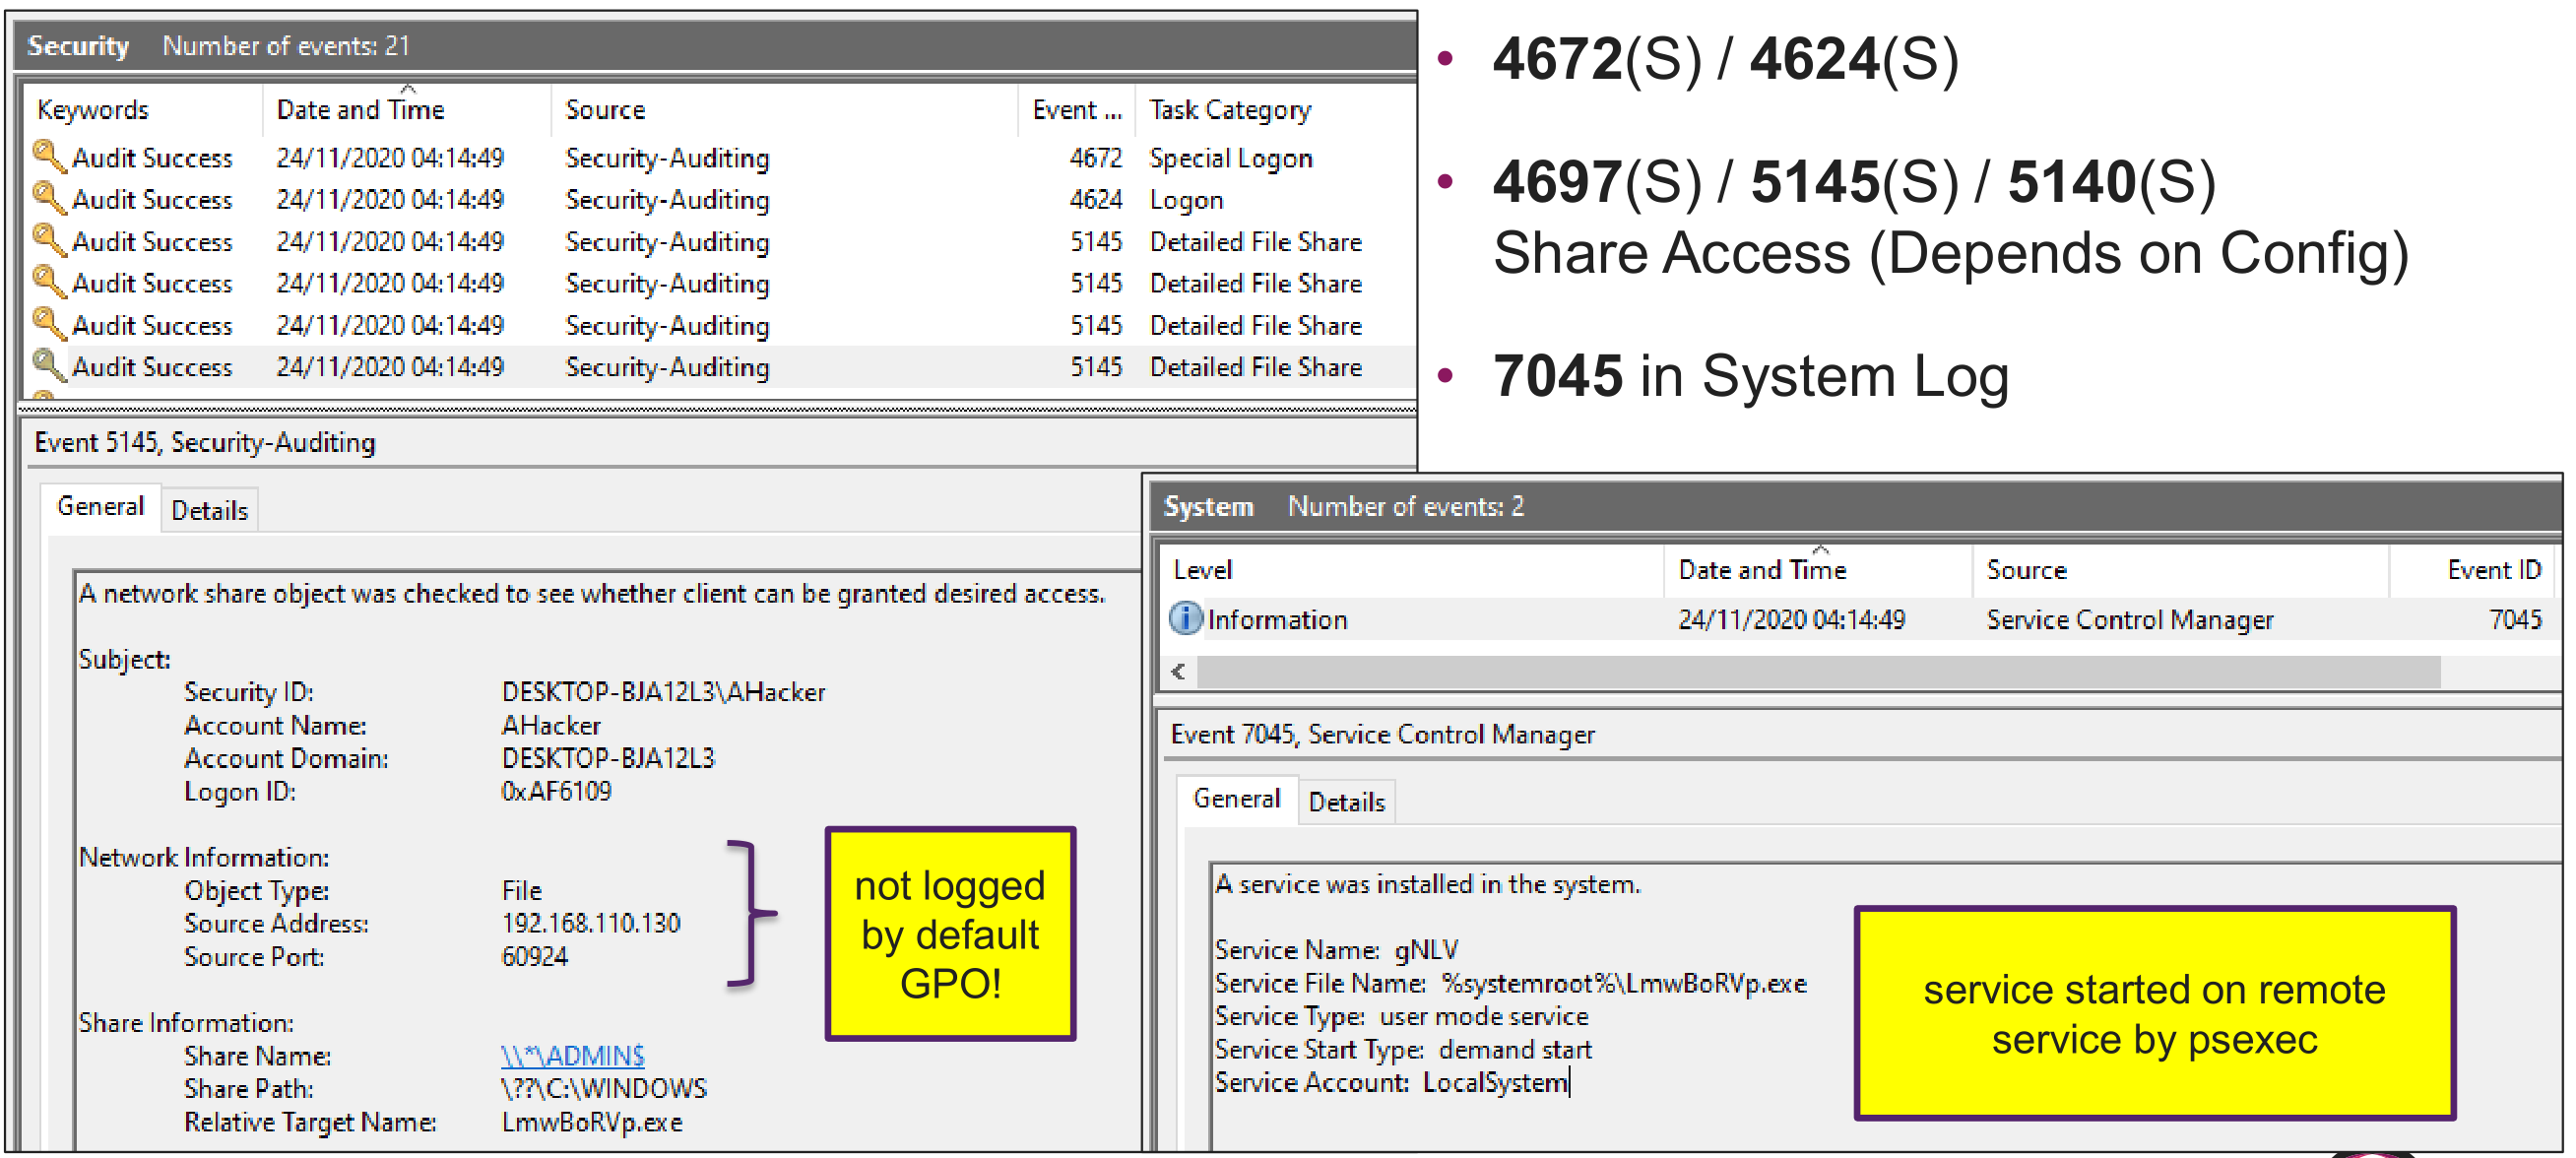
\includegraphics[width=\linewidth]{event-log-lateral-movement.png}

\subsubsection{Scheduled Tasks}
\begin{itemize}
  \item 4698: A scheduled task was created
  \item 4700: A scheduled task was enabled
\end{itemize}

\subsubsection{PowerShell Event Logs}
PowerShell/Operational Log holds the most data:
\begin{itemize}
  \item 4103 Module/Pipeline output logging
  \item 4104 Script block logging
  \begin{itemize}
    \item PowerShell Version 5+ has extensive logging
    \item Automatic logging of suspicious scripts: 4104 with Warning Level.
  \end{itemize}
  \item Often Obfuscated Payloads
\end{itemize}

\paragraph{PowerShell.evtx}
PowerShell.evtx is older and may hold some data.
\begin{itemize}
  \item EID 400: The engine status is changed from None to Available. This event indicates the start of a PowerShell activity, whether local or remote.
  \item EID 600: Provider ``XYZ'' is Started. Indicates that providers such as WSMan start to perform a PowerShell activity on the system, for example, “Provider WSMan Is Started”.
  \item EID 403: The engine status is changed from Available to Stopped. This event records the completion of a PowerShell activity.
  \item HostName field in message details. 
  \begin{itemize}
    \item For a local activity: HostName = ConsoleHost
    \item Remote activity: HostName = ServerRemoteHost (on the system that is accessed)
  \end{itemize}
\end{itemize}

\paragraph{Logging in PS}
PSReadline: Records last 4096 typed commands (Enabled by default)
\begin{lstlisting}
  %appdata%\Microsoft\Windows\PowerShell\PSReadLine\ConsoleHost_history.txt
\end{lstlisting}
Transcript Logs: Logs PS input and output at the terminal (Disabled by default)
\begin{lstlisting}
  #Can be enabled with:
  Start-Transscript / GPO
  #Located under:
  %userprofile%\Documents
\end{lstlisting}

\subsubsection{USB Devices}
Devices and their device drivers appear in the Device Manager MMC snap-in.
\paragraph{System.evtx}
\begin{itemize}
  \item 10000 DriverFramework-Usermode - driver package is being installed.
  \item 10100 DriverFramework-Usermode - the driver package installation has succeeded.
  \item 20001 User Plug-n-Play Device Event - Device Installation.
\end{itemize}
\paragraph{Microsoft-Windows-NTFS\%4Operational.evtx}
142 - Free space on the drive and the volume name
\paragraph{Microsoft-Windows-Partition\%4Diagnostic.evtx}
1006